%
\chapter{Grouping and labeling}
%
We want to be able to distinguish between different types of scenes so that we have a way to structure the final video summaries. We apply a label to each frame in a video, using a label-classifier, and then group consequtive frames with the same label.
%
\section{Literature Study}
%
There are many ways to extract context from images, sound and video. Some focus on the depicted scene itself, while others look at the events happening in the scene. Location and time of day would be an example of the former while elements such as excitement, violence and other specific behaviour are examples of the later.\\
Hanjalic\cite{citeulike:405480} describes a way to identify regions of high levels of excitement in sports videos based on a manually selected set of features. These features can be both visual (e.g. movement in an image or change of camera position) or audial (based on the energy contained in the audio track).\\
Optical Flow, as described by Bouguet \cite{Bouguet2000}, can also be used to detect events or objects in video. Optical Flow analyses changes in the intensity pattern in images. In many cases this indirectly indicate changes in the 3D scene caused by moving objects or a change of view-point. \cite{mangler} describes ways to identify certain types of actions occuring within videos, such as violent behaviour and \cite{mangler} looks at general crowd movement in public places.\\
% Lauge: Der skal skrives lidt mere til disse artikler.
Reisman et al. \cite{CrowdDetectionInVideoSequences} describes a way to identify crowds of pedestrians from a moving vehicle by detecting inward moving optical flow. I.e. flow which is highly likely to be caused by moving objects and not due to a change of view-point.\\
Arandjelović \cite{Arandjelovic08crowddetection} attempts to identify crowded regions in still images based on the hypothesis that crowds contain a certain general structure, namely that an image with crowds in it will contain regions, which at a close scale resembles individual people, while at a larger scale will contain repetative structures.\\
Zhong et al. \cite{10.1109/CVPR.2004.78} describes a technique for unsupervised detection of unusual events in a video stream. The entire stream is divided into overlapping 4 second segments from which an overall movement pattern is established. Individual segments that differ too much from this patter are considered unusual.\\
% Lauge: Day/Night article her skal uddybes og omskrives:
In \cite{mangler} ?HVEM? describes how to classify still images through a hierachy of Support Vector Machines, including day/night classification. UDDYB\\
Angin et. al \cite{10.1109/MDM.2010.71} describes a method of automatically detecting the color of traffic lights. UDDYB % Lauge: Vi skal lige have læst/skrevet lidt mere om denne og evt. relation til police blinker detecion
%
\section{Method}
%
The labeling happens in two phases. First we extract different kinds of metadata from the individual videos. This is done frame-by-frame, for each type of metadata, so we end up with a collection of describing properties throughout each video. Some of the metadata is directly available from the earlier phases of the project. The level of \textit{contrast ratio} and the \textit{shift vector magnitude ratios} described in section \ref{sec:frame_shift_estimation} and \ref{sec:frame_contrast_estimation} and revisited below in sections \ref{sec:contrastdata} and \ref{sec:svmdata}, are examples of this. We use the frame mean pixel intentisity to estimate overall brightness (section \ref{sec:brightnessdata}) and seperate the blue color channel (section \ref{sec:blue_channel}). People detection (section \ref{sec:peopledata}) is done using Haar cascade classifiers and Optical flow (section \ref{sec:opticalflowdata}) is used for extracting additional event information.\\
\\
The actual labeling is subsequently done by analysing the metadata using a collection of classifiers. Section \ref{sec:police_detection} describes a \textit{police blinker} classifier, which identifies oscillation in the blue channel from the individual frames. Section \ref{sec:overviewclassifier} describes an \textit{overview} classifier, which attempts to detect footage containing little egomotion (camera movement). In section \ref{sec:verticaloscillationclassifier} we attempt to identify vertical oscillating movement in the optical flow, using it as an indicator for people jumping or signs being lifted into the air. Section \ref{sec:incrowd} describes an \textit{in-crowd} classifier, which uses facial- and person- detection to detect footage with several people in it. In section \ref{sec:infocus} we further explore the area of people detection, by looking for footage, which focuses on a specific (assumably interesting) person for a duration of time. Finally, in section \ref{sec:daynightclassifier} we look at differentiating between day- and night- time footage by working with the different brightness and color intensity metadata we have extracted.
%
\subsection{Haar Cascade Classifier}\label{sec:hcc}
%
The Haar Cascade Classifiers (HCC)\cite{viola01,lienhart01,schmidt01,schmidt02} classifies Haar-like features, which is an efficient way of detecting specific objects in an image. A Haar-like feature describes how to categorize subsections of an image, where the categorization is based on the difference in sums of pixel intensities in adjancent regions. For ex. in an average human face the eye-region is generally darker than the cheeks, hence if two adjacent regions is the eyes and the cheeks. then there should be a significant difference in pixel intensity sums of these two regions, indicating a human face. Ie. this difference and the relative position of the two regions makes up a Haar-like feature.\\
% A Haar-like feature considers adjacent rectangular regions at a specific location in a detection window, sums up the pixel intensities in each region and calculates the difference between these sums. This difference is then used to categorize subsections of an image. For example, let us say we have an image database with human faces. It is a common observation that among all faces the region of the eyes is darker than the region of the cheeks. Therefore a common haar feature for face detection is a set of two adjacent rectangles that lie above the eye and the cheek region. The position of these rectangles is defined relative to a detection window that acts like a bounding box to the target object (the face in this case).
HCC uses a data-structure called an integral image, an algorithm based on AdaBoost that selects critical visual features, and a method that combines complex classifiers to compute on the most promising object-like regions. Initial results by Viola\cite{viola01} achives 15 frames per second detection in an 384 by 288 pixel image using, by todays standards, outdated hardware.\\
%
An integral image (aka. summed area table) is a matrix where any point $(x,y$ is the sum of all pixels above and to the left of $(x,y)$ illustrated in Figure \ref{fig:integral_img} where the area of $\square ABCD$ can be computed as $S=A-B-C+D$, ie. the sum of any subpart of the integral image can be quickly determined. Not only is the computation of this matrix efficient as a function of its nature (it can reuse already computed sums when building the matrix), the sum at any given point can be computed in constant time as it can be done by 4 lookups in the matrix followed by 4 additions/substractions. When detecting Haar-like features the region sums can be computed efficiently using this datastructure.
%
\begin{figure}[!ht]
     \centering
     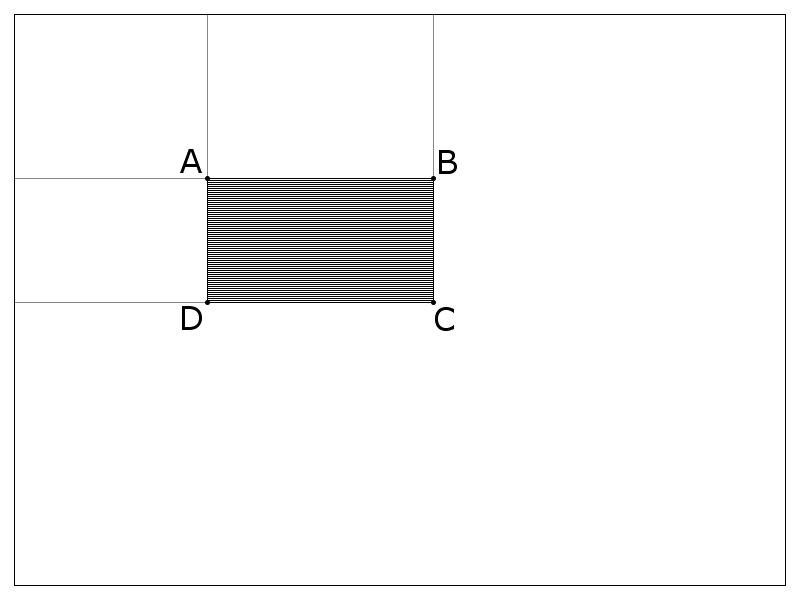
\includegraphics[width=0.50\textwidth]{img/integral_image.png}
     \caption{Integral image}\label{fig:integral_img}
\end{figure}\\
%
AdaBoost (Adaptive Boosting) is a meta-algorithm for boosting machine learning algorithms where subsequent classifiers built are tweaked in favor of those instances misclassified by previous classifiers. The derivative algorithm is a modification of AdaBoost that constrains each returned (weak) classifier to be dependent only on a single feature, which in turn is deemed a critical feature.\\
HCC also employs a method of using less complex processing to detect promising regions, the rationale being that it is often possible to rapidly determine where an object may occur within an image, and then apply the more complex processing on these regions.
%
\subsection{Optical Flow}
%
For analysing internal movement within the frames, we use the pyramidal implementation of the Lucas Kanade Feature Tracker described by Bouguet\cite{Bouguet2000} (supplied by OpenCV).\\
Optical flow is a tool for detecting how individual pixels move around between consecutive frames $I$ and $J$. If $(x,y)$ is the position of a pixel in $I$, this is done searching for the pixel at position $(x+d_x,y+d_y)$ in $J$, which is most similar. The optical flow of $x$ is defined as the $d=(d_x,d_y)$, for which the difference in pixel intensity is smallest. The search is done in a search window around the original position. The size of this window determines the trade-off between precision and robustness.\\
The pyramidical implementation creates several \textit{levels} of images, each level halfing the resolution of them. Starting with the smallest resolution images, an estimation of the optical flow is performed. This estimation is then passed to the next level, where it is improved. This is repeated all the way up to the orginal images, where the final optical flow vector is computed.
%
\subsection{Metadata}
%
This section describes the different type of metadata we extract.
%
\subsubsection{Contrast}\label{sec:contrastdata}
%
The \textit{contrast} in a frame is defined as being the standard deviation of the intensity values in the image-matrix, as described in section \ref{sec:frame_contrast_estimation}. A small deviation would indicate little contrast/diversity in color-intensity, and a large deviation would indicate a high contrast/much diversity in intensity. The \textit{contrast} metadata for each video consist of the set of these standard deviations for each frame.
%
\subsubsection{Shift vector magnitude}\label{sec:svmdata}
%
Like the contrast, the \textit{shift vector magnitudes} for each video is already computed as a part of the initial image quality assessment, as described in section \ref{sec:frame_shift_estimation}. We make a rough estimation of the egomotion (camera movement) by shifting all pairs of neighbouring frames until they align. This shift is expressed as a vector, whos magnitude tells us how much the camera is moving/shaking at each frame point in the video. The \textit{shift vector magnitude} metadata consists of set of these magnitudes throughout the video. It is used in the \textit{overview} classifier described in section \ref{sec:overviewclassifier}
%
\subsubsection{Brightness}\label{sec:brightnessdata}
%
The \textit{brightness} metadata consists of the mean pixel intensity in each frame throughout the video. It is used in the \textit{day/night} classifier described in section \ref{sec:daynightclassifier}.
%
\subsubsection{Blue color channel}\label{sec:blue_channel}
%
This particular type of metadata is extracted from the original videos (before grayscale conversion). Each frame in a video consists of a matrix of pixels in 3 channels; red, green, and blue. We extract the blue channel for the purpose of police blinker detection, described in detail in section \ref{sec:police_detection}, and day/night detection, described in detail in section \ref{sec:daynightclassifier}.
%
\subsubsection{The presence of people}\label{sec:peopledata}
%
Detecting the presence of people will help us determine if footage was recorded from within a crowd, described in detail in section \ref{sec:incrowd}, or if the footage has focus on a specific person, described in detail in section \ref{sec:infocus}, which indicates that this person is of special interest, ex. a speaker.\\
%
OpenCV provides a python-implementation of an already trained Haar Cascade Classifier, as described in section \ref{sec:hcc}, manifested as a range of xml-files describing the Haar like features of a human face, both front and profile, aswell as upper body, lower body, and full body.\\
By deploying facial detection to every frame in each video we get a good estimate of how many people are present, and also their location within each frame. This estimate is limited by the quality of the frame, ex. shaky video-clips have a reduced detection rate.\\
%
A possible optimization is to only analayze select frames (ex. every third frame) which we do not believe will have a significant negative impact on the detection rate as we already interpolate the detected objects from frame to frame. Further optimizations involve exploiting the ready-at-hand metadata, such as the general frame quality which severely impacts facial detection rates.\\
A more complex optimization can be achived by exploiting the temporal data. Ie. instead of analyzing the entire frame using an expanding search window, we could utilize knowledge of where people were present in the previous frame, and then deploy the search window nearby. This would require a customized HCC which is a major increase in complexity compared to the other mentioned optimizations.
%
% MOVE TO RESULTS:\\
% we also experienced a significant increase in false positives for banners and flags (which there is a presence well above normal in our training set). We are working with 480 by 640 pixel images and are able to achieve real-time facial detection (working on video with 24 frames per second).\\
%
\subsubsection{Internal movement}\label{sec:opticalflowdata}
%
Where \textit{shift vector magnitudes} tells us something about how the camera itself moves, the internal movement in a frame (computed using optical flow) attempts to explain how the content within each frame moves. A lot of research has been done on this subject. Unfortunately, most of the existing work done on both event- and crowd- classification focuses on settings with stationary cameras. Although Reisman et al. \cite{CrowdDetectionInVideoSequences} \textit{do} work with images from a camera fixed on a moving vehicle, their appraoch is still not applicable to our scenario, since our videos are recorded mostly by handheld devices, whose movement are a lot less predictable. Extracting the internal movement of our videos is therefore not only a matter of analysing how reference points move around in the frame. First we must estimate the \textit{egomotion} (the motion of the camera) itself, in order to \textit{stabilise} the frame.
%
\paragraph{Frame stabilisation}
%
There are several ways to do this. An option is to use the \textit{shift vector magnitudes} that we have already computed. This intuitively makes sense since they are suppose to describe the movement of the camera at at each frame in the video. However, it turns out that although this data may be suitable for describing the general type of cameara movement (shaking, panning), especially when the data is smoothed across several frames, it has a relatively high margin of error for individual frames. This is especially the case if the camera moves very fast or if there actually \textit{is} a lot of movement within the frame. Another option is use the mean of all the optical flow vectors as the egomotion. Alternatively one could use the most commonly occuring vector. However, our experimentation showed that these two methods suffer from one serious limitation. If moving objects in the frame are very close to the camera, they tend to become more influencial than the stationary background and they end up swapping roles. The egomotion is then based on the movement of the large object, the opposite of what we want. The border-case for this condition is especially problematic. This occurs when a moving object takes up half of the frame. Often, changes in position will then \textit{periodically} cause it to be more or less dominant than the background. In these cases the egomotion vector will jump from one extreme to the other, in close succession, and thus become completely useless.\\
Some of these problems could probably be alleviated through further analysis or averaging across time. However, through our experimentation we came up with an approach that seems more promising.\\
\\
\textit{Corner detection} refers to identifying features in a frame, which are \textit{good to track}. They are areas (or points), which are likely to be clearly distinguishable on the following frames. This is often done by locating areas with low \textit{self simmilarity}. That is, areas that do not look like other areas close by. We found that generally, these points has a tendency to be present in stationary objects in the frame far more often than in moving objects, and thus form a very decent base for our egomotion vector. The implementation we use to identify these features is based on the Shi-Tomasi corner detection algorithm described by Shi et al. \cite{Shi_1994_3266}. We track these features and define our egomotion to be the mean of all the resulting displacement vectors.\\
\\
Note: We have later come across other, more advanced techniques for calculating the egomotion of a video. Raudies et al. \cite{Raudies:2009:ELM:1612122.1612125} describes such a method. Unfortunately, do to our late discovery of this method we have not been able to test it.
% Lauge: Der skal skrives noget mere om denne metode, hvis den skal nævnes, desuden skal dette rykkes til future work
%
\paragraph{Detecting movement}
%
We now look at the movement within the frames. We place a grid of points across the frame and perform optical flow analysis on them. We use a pyramidal implementation of the Lucas Kanade feature tracker described by Bouguet\cite{Bouguet2000}. We do the analysis with a grid of 24x16 points, using a search window of 30x30 pixels over two pyramidical levels.\\
Some of the resulting vectors are discarded if the feature tracking was unsuccessful. This is often the case with features in the sky or in surfaces without any distinct features, or if the point being tracked ends up outside of the following frame.\\
For every vector $v \in V$, where $V$ is the set of valid displacement vectors, the isolated movement vector $v'$ is defined as:
\begin{equation}
v' = v - e,
\end{equation}
where $e$ is the egomotion vector for the frame. The set of all $v'$ then describes the internal movement of objects within the frames.\\
Each vector $v' \in V'$ describes the movement of one particular point in the original grid. By looking at the different directions of flow we may be able to say something about what is going on in the video. To simplify the data we divide the optical flow vectors up into nine segments as shown in figure \ref{fig:opticalflow}. We calculate the mean of the movement vectors in each group, seperately, and use these nine new vectors to describe the overall flow in different parts of the frame.
%
% Lauge: RISK - This model may be too simple, for good results
%
\begin{figure}
     \centering
     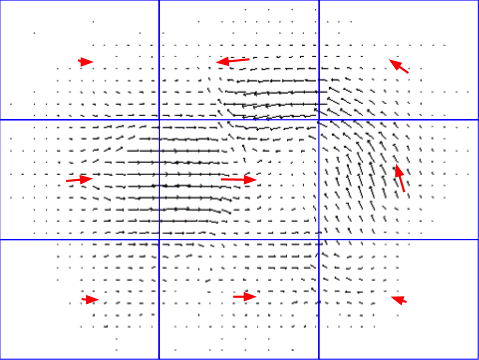
\includegraphics[width=0.75\textwidth]{img/optical_flow.png}
     \caption{Example of optical flow vectors in a frame. The red arrows shows the overall flow within a segment of the frame}\label{fig:opticalflow}
\end{figure}
%
The \textit{optical flow} metadata consist of sets of these nine vectors, calculated for each frame in the video. It is used in the \textit{vertical oscillation} classifier described in secion \ref{sec:verticaloscillationclassifier}.
%
\subsection{Label classifiers}
%
A label classifier performs a binary classification on each frame in a given video. For each video the classifier computes groups of consecutive frames with the same label. Such a group is called a segment. Depending on the classifier, the segments are post-processed using \textit{segment interpolation} and/or \textit{segment smoothing}. Some classifiers have this as a builtin feature.
%
\subsubsection{Segment Smoothing}\label{sec:labelsmooth}
%
If segments from the same video are fragmented we apply triangle smoothing on the segments, as described in section \ref{sec:triangularsmoothing}. Prior to smoothing each frame had either a 1 (label present) or a 0 (label not present), but post-smoothing they are a fraction between 0 and 1. These values are subsequently truncated to 0 if they are below a certain treshold.
%
\subsubsection{Segment Interpolation}\label{sec:labelmerge}
%
Segments in a video are easilly fragmented and two segments with the same label just a single frame apart will by all means and purposes be interpreted as such. We interpolate neighbouring segments by applying the label, $l$, to the frames between segment $a$ and segment $b$ if these are not too far apart and both segments share the same label, $l$.
%
\subsubsection{Police Blinker Classifier}\label{sec:police_detection}
%
By investigating the blue channel mean of each frame (section \ref{sec:blue_channel}) we are able to detect if police blinker lights are present in part of a video.
We analyze the blue channel mean as a function of time, and if these values are oscillating with a steady frequency we have an indication of the presence of police blinker lights.
%
\begin{figure}[!ht]
     \centering
     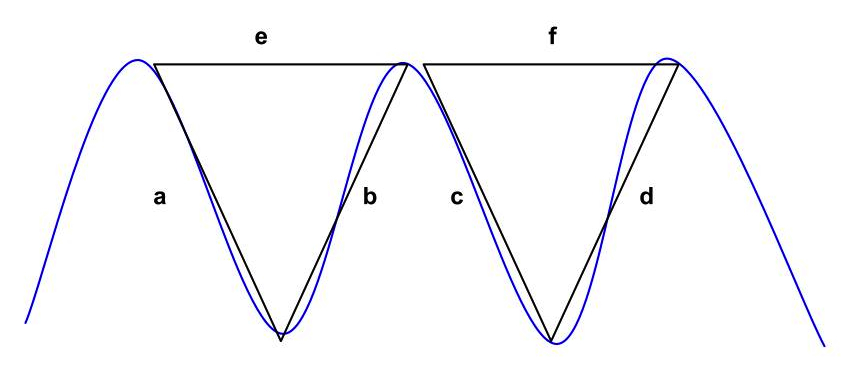
\includegraphics[width=1.05\textwidth]{img/triangles.jpg}
     \caption{}\label{fig:triangles}
\end{figure}\\
% Lauge: Mangler title
Local minima/maxima in an oscillating graph connected by straight lines will form triangular shapes as illustrated in Figure \ref{fig:triangles}, where consequtive triangles of roughly equal size indicate a steady oscillation. We investigate if the length of the vertices in each triangle deviate from each other
\[
\text{std}([\|a\|,\|b\|,\|c\|,\|d\|]) < \tau_1, \text{std}([\|e\|,\|f\|]) < \tau_2,
\]
% a,b,c, og d skal defineres i tekst
for thresholds $\tau_1$ and $\tau_"$ where std is the standard deviation. If the standard deviation of either group of vertices is below their given treshold it means that they do not form triangles that are part of an oscillation.\\
The blue channel mean is smoothed using triangle smoothing as described in section \ref{sec:triangularsmoothing}, as this results in softer curves on the graph. Oscillating segments are then detected, and nearby segments are merged as described in section \ref{sec:labelmerge}.
%
\subsubsection{Person in Focus classifier}\label{sec:infocus}
%
We compute a moving average of the people presence metadata, but excluding objects detected (partially) outside a centered bounding box. Then the frames and their respective label are smoothed as described in section \ref{sec:labelsmooth}, and nearby segments are merged as described in section \ref{sec:labelmerge}. 
% segments shorter than 120 frames, equal to 5 seconds, are removed.
%
\subsubsection{In-Crowd classifier}\label{sec:incrowd}
%
We compute a moving average of the people presence metadata to determine if the frame is shot from within a crowd, or slightly overlooking a crowd. The frames and their respective label are smoothed as described in section \ref{sec:labelsmooth}. Nearby segments are merged as described in section \ref{sec:labelmerge}.
%
\subsubsection{Overview classifier}\label{sec:overviewclassifier}
%
The \textit{overview} classifier attempts to detect footage with negligible egomotion, as well as little internal movement within the frames. In order to avoid overlap with the \textit{person in focus} footage, which often share these characteristics, we also require the overview footage to not focus on any person in particular. The overview classifier uses the shift vector magnitude metadata described in section \ref{sec:svmdata}, the optical flow metadata described in section \ref{sec:opticalflowdata}, as well as the actual labels classified by the \textit{person in focus} classifier described in section \ref{sec:infocus}.\\
We perform a slight triangular smoothing on the metadata in order to remove outliers. We also desregard all footage, which has already been classified with the \textit{person in focus} label.\\
We now look at the amount of movement in each area of the image in order to determine if a frame contain too much internal movement. Let the internal movement in a frame be defined as $f = [m_{1},m_{2} \dots m_{9}]$, where $m_{i}$ is mean distance of movement occuring in a specific area the frame. This mean is calculated on the magnitude of all adjusted optical flow vectors, in that area. The number of areas exceeding a given threshold, $\tau_{1}$, is then defined as:
%
\begin{equation}
A(f) = \sum_{i=1}^{9}
\begin{cases}
0 & \text{if } m_{i} \leq \tau_{1}\\
1 &  \text{otherwise}
\end{cases}
\end{equation}
%
Calculating individual means and analysing each area seperately, should improve the chance of detecting local characteristics, which could otherwise have been lost in a global mean.\\
 Next we combine this meassure with the egomotion, $f_{e}$, as estimated by the shift vector magnitude, at this frame. The binary \textit{overview} classification of a frame is defined as:
\begin{equation}
O(f) =
\begin{cases}
0 & \text{if } A(f) > \tau_{2} \vee f_{e} > \tau_{3} \\
1 &  \text{otherwise}
\end{cases},
\end{equation}
where $\tau_{2}$ is a threshold that defines how many areas are allowed to exceed the internal movement limit, and $\tau_{3}$ is a threshold defining the maximimum shift vector magnitude we accept for the frame.
%
\subsubsection{Vertical Oscillation classifier}\label{sec:verticaloscillationclassifier}
%
The \textit{vertical oscillation} classifier attempts to detect footage with vertical movement of objects. Such movement can be caused by people jumping, by people gesticulating heavily whilst talking, or by signs being raised into the air. We look at the variance of the vertical direction of the optical flow vectors over some period of time.\\
As with the \textit{overview} classifier we analyse the internal movement in different areas of the image, in order to detect local characteristics. Let $m$ be the mean of the vertical movement in an area of a frame. This mean is calculated on the vertical movement of the adjusted optical flow vectors, in that area. The variance in vertical movement in an area of the image at frame position $f$ is then defined as:
%
\begin{equation}
v(f) = std \left (\bigcup_{i=f-\tau_1}^{f} m(i) \right ),
\end{equation}
%
where $\tau_1$ is the timespan over which we want to calculate the variance. For simplicity we omit the case where $f \leq \tau_1$. In that case we let $v_{f} = 0$.\\
Let $V$ be the set of all nine image areas in a video. The number of areas, in a frame at position $f$, in which vertical oscillation occurs is then defined as:
%
\begin{equation}
A(f) = \sum_{i=1}^{9}
\begin{cases}
0 & \text{if } V_{i}(f) < \tau_2\\
1 &  \text{otherwise}
\end{cases}
\end{equation},
%
where $\tau_2$ is some threshold defining the minimum level of variance. The \textit{vertical oscillation} classification of a frame is then defined as:
%
\begin{equation}
V(f) =
\begin{cases}
0 & \text{if } A(f) < \tau_3\\
1 &  \text{otherwise}
\end{cases},
\end{equation},
%
where $\tau_3$ is a threshold defining the minimum number of areas in which vertical oscillation must occur.
%
% RISKS: (zooming), maybe wrong method
%
\subsubsection{Day \& Night classifier}\label{sec:daynightclassifier}
%
Night footage is not only darker than footage recorded during the day, it also contains significantly less blue color, which is the reason it often has a brownish or red tint. Our \textit{day/night} classifier analyses both the \textit{blue channel} metadata (described in section \ref{sec:blue_channel}) and the \textit{brightness} metadata (described in section \ref{sec:brightnessdata}).\\
First, we look at the correlation between the blue color channel and the overall brightness. Let $i$ be the frame position in the video, and let $R$ and $L$ be the set of brightness- and \textit{blueness}- values for all frames, respectively. Then the correlation $c_{i}$ is defined as:\\
%
\begin{equation}
c_{i} = \frac{L_{i}}{R_{i}} - 1
\end{equation}
%
A value above zero shows that blue is a dominant color in the frame.\footnote{We have later discovered that, due to the way images are converted to greyscale, this is not always true. We describe this problem in detail in the Discussion section for this chapter (section \ref{sec:phase2discussion})}
$c$ is therefor an indication of what type of footage we are dealing with.\\
Next, we look at the general distribution of brightness intensities throughout the video. We start by creating a histogram of the brightness distribution across the entire video. The histogram have a range of [0:255] and contain $b$ bins of equal size. For each frame in the video, the mean brightness value is inserted into the histogram. Figure \ref{fig:brightness_histogram} shows an example of this mapping.
%
\begin{figure}
     \centering
     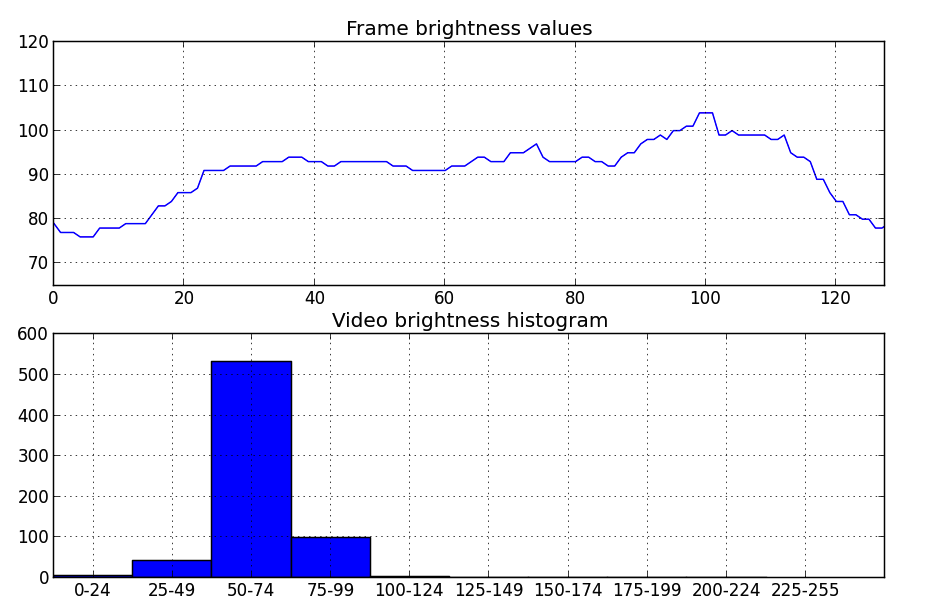
\includegraphics[width=1\textwidth]{img/brightness_histogram.png}
     \caption{Example of frame brightness intensities being mapped to a histogram.}\label{fig:brightness_histogram}
\end{figure}
%
Now we look at this histogram and compare the mass of the partitions representing the darker frames with the mass of those representing the brighter ones. Let $H$ be the histogram for a video, and let $\tau \in \{1,2,...,b-1,b\}$ be some delimeter value. An indication of daytime is then defined as:
%
\begin{equation}
D = \sum_{i=1}^{m}H_{i} < \sum_{j=m+1}^{10}H_{j}
\end{equation}
%
Finally, let $C$ be the mean of all $c$ in a video. Our \textit{day/night} classifier is then defined as:
\begin{equation}
S =
\begin{cases}
\text{day} & \text{if } C > 0 \vee D \\
\text{night} &  \text{otherwise}
\end{cases}
\end{equation}
%
% \section{Dataset}
% %
% Here we should have a brief explanation of what videos are in our dataset.
%
\section{Findings}
%
This section describes the parameter tuning of the classifiers along with some informal performance statistics. In general all tuning is done through emperical testing. These parameters should therefore only be seen as a starting point for more extensive research. Unless otherwise noted, tuning is done on a small subset of the dataset. The entire dataset consists of 131617 frames ($\sim$ 90 minutes) of footage. For all, but the \textit{day/night} classifier, performance is meassured only in true positives/false positives. We derive the results from manual observation of the classified segments, where each classification is determined to be either correct or wrong.\\
%
PEOPLE DETECTOR:\\
we also experienced a significant increase in false positives for banners and flags (which there is a presence well above normal in our training set). We are working with 480 by 640 pixel images and are able to achieve real-time facial detection (working on video with 24 frames per second).\\
%
\subsection{Segment Interpolation and Smoothing}
%
When interpolating segments we require that two neighbouring segments (direct neighbours) are within a certain distance in order to be valid candidates for interpolation. Unless otherwise noted, this distance is 24 frames.\\
When smoothing the segments with triangular smoothing we found that a degree of 36 gave reasonable results. This roughly corresponds to smoothing over 3 seconds of video footage. Unless otherwise noted values less than $1/3$ are truncated as described in section \ref{sec:labelsmooth}.
%
\subsection{Police Blinker classifier}
%
Before we investigate if the blue channel mean is oscillating, we smooth the values with a smoothing degree of 5 to get slightly smoother curves, but still retaining much of the original data.\\
The segments are also interpolated, as described in section \ref{sec:labelmerge}, but we interpolate segments up to as much as 48 frames apart, instead of the standard 36.
%
We meassure performance based on how many of the classified segments contain police blinkers or actually has police personal present in the footage. We include the latter scenario because the light from police blinkers off-screen may be detectable in the blue color channel, even if it is not visible to the human eye.\\
Out of the total $\sim$ 90 minutes of footage 699 frames $\sim$ 30 seconds are classified positive. Of this $\sim$ 65\% are what we consider \textit{true positives}. % Lidt her om false positives. Hvad er grunden til dem?
%
\subsection{Person in Focus classifier}
%
When computing the moving average over people presence metadata, we do it over 4 frames. This means that the data needs to be fairly consistent already in order to get a consistent detection, ie. just a few frames with no person detected within the centered bounding box would diminish the moving average towards zero.\\
%
We meassure performance based on how many of the classified segments has a specific person in focus. Segments with several people or crowds are considered incorrectly classified.\\
Almost 21 minutes of the entire dataset is classified as containing a person in focus. Hereof we consider $\sim$ 90\% to be \textit{true positives}.
%
%
\subsection{In-Crowd classifier}
%
When computing the moving average over people presence metadata, we do it over 12 frames, which roughly translates to half a second. This allows for some inconsitency in the people presence metadata. The labels are smoothed using a smoothness degree of 24 which SOMETHING WITH MOVING AVERAGE. The values are truncated at 0.9 as they are not normalized to the range 0 to 1 as our data often is.
%
A fallacy in this method are cases of just two people in a frame which are easily detectable, ie. facing a steady camera with no background clutter.\\
\\
We consider footage recorded within a crowd, or in close proximity to several people, to be \textit{true positive} \textit{in-crowd} clips. Approximatly 14\% of the $\sim$ 31 minutes of positively classified footage fulfills this requirement. The vast majority of the \textit{false positives} are caused by persons in focus.
%
% Til analyse: In hindsight we should have expected the \textit{person in focus}-issue to be a problem.
%
% Til phase 4: Due to the \textit{person in focus}-issue with in-crowd shot we attempt to do correction by forbidding the former label in the latter shots :P
%
\subsection{Overview classifier}
%
The \textit{overview} classifier (described in section \ref{sec:overviewclassifier}) analyses both the internal movement in the frames, as well as the overall egomotion of the camera.\\
The classifier has three thresholds, $\tau_{1}$, $\tau_{2}$ and $\tau_{3}$. $\tau_{1}$ is the maximum internal movement allowed in an area. $\tau_{2}$ is the maximum number of areas, which are allowed to break this limit, and $\tau_{3}$ is the maximum allowed egomotion for the entire frame.\\
The parameter tuning was done a small subset of the dataset, consisting of a handful of videos. Setting $\tau_{1} = 2 \text{ pixels}$ and $\tau_{2} = 2 \text{ areas}$, seems to ensure sufficiently low levels of internal movement. Setting $\tau_{3} = 10 \text{ pixels}$ appears to keep unsteady camera movement at a minimum, while still allowing for panoramic movement, which we do not want to discard.\\
Lastly, for the triangular smoothing of the metadata a triangle width of 120 frames is used. We have not performed any tuning on this parameter.\\
\\
It is difficult to exactly define what an \textit{overview} clip is. These are the charactaristics we look after when determining performance:
%
\begin{itemize}
	\item \textbf{Detachment from events}: The camera is not affected by the events being filmed. The camera is not affecting the events.
	\item \textbf{Scene depiction}: The footage shows the scene itself, not specific events in the scene. For this reason we do not accept footage of persons in focus.
	\item \textbf{Quality of footage}: The footage actually shows something. Footage depicting the sky or a close up shot of someones back, is not accepted.
\end{itemize}
%
As a rule of thumb, we consider segments fulfulling these requirements \textit{true positives}. In total $\sim$ 22 minutes are classified as being . Of these $\sim$ 43\% are considered correct. When reviewing the segments we clearly see that a lot of the \textit{false positives} are caused by clips with a \textit{person in focus}. This is a clear indication that our attempt to mutually exclude the two labels is failing.
%
\subsection{Vertical Oscillation classifier}
%
The \textit{vertical oscillation} classifier (described in section \ref{sec:verticaloscillationclassifier}) analyses the internal movement in the frames.\\
It has three thresholds. $\tau_1$ defines the time span over which the standard deviation in vertical movement is calculated. $\tau_2$ defines the minimum level of variance accepted as vertical oscillation. $\tau_3$ defines the number of areas in the frame in which vertical oscillation must occur.\\
The parameter tuning is done on on a small subset of the dataset (3-4 videos). For the variance coverage we set $\tau_1 = 12 \text{ frames}$, representing half a second of footage, enough for someone to jump or make a gesticulation. The minimum amount of variance required is set to $\tau_2 = 5 \text{ pixels}$, which, over 12 frames, will require significant vertical oscillation in order to be achieved. Because vertical oscillation only is required in a small part of the frame in order to be clearly visible, we set $\tau_3 = 2 \text{ areas}$.\\
As with the \textit{overview} classifier, we smooth the metadata with a trinagle width of 120 frames.\\
\\
When analysing the performance of the \textit{vertical oscillation} classifier, segments depicting objects being moved up and down are considered \textit{true positives}. In total $\sim$ 14\% of the 8 minutes of the positively classified footage fulfills this requirement. A review show that the vast majority of \textit{false positives} are caused by unsteady camera motion, which we fail to compensate for. Groups of people walking also trigger a lot of \textit{false positives}, which suggest an over-sensitivity to vertical movement.
%
% Til analyse: A pre-limmenary image quality assesment might help in lowering the amount of \textit{false positives}.
%
\subsection{Day \& Night classifier}
%
The \textit{day/night} classifier (described in section \ref{sec:daynightclassifier}) analyses the overall brightness in a video along with the blue channel.\\
It has two parameters. $b$ is the number of bins in the histrogram of brightness intensities, and $\tau \in \{1,2,...,b-1,b\}$, which determines where to make the differentiation between the dark and bright partitions in the histogram. We let $b = 10$ and subsequently tried all 10 values of $\tau$. We find that $\tau = 3$ yields the best results. The parameter tuning is done on the entire dataset and is thus almost certainly overfitted.\\
\\
The classification is performed on 301 video-clips where $\sim$ 88\% of them contain daytime footage. Using this parameter we are able to correctly classify videos with $\sim$ 97\% accuracy. And even then, many of the false classification occur in videos in the evening or the late afternoon, which are difficult to classify, even manually.
%
\subsection{Analysis}
%
\subsection{Discussion}\label{sec:phase2discussion}
%
The \textit{overview}- and the \textit{person in focus}- labels are defined to be mutually exclusive. In case of a overlap the latter is used. However, due to the order in which the labels are generated and post-processed, overlaps \textit{can} actually occur. Because the \textit{person in focus} labels are interpolated (as described in section \ref{sec:labelmerge}) only after the the \textit{overview} classifier have used them for its classification, the new, interpolated \textit{person in focus} labels may actually cover areas which are also labelled as overviews.\\
\\
In the \textit{day/night} classifier we compare the blue channel intesity of a frame with the overall brightness, in order to determine if blue is a dominant color. However, the overall brightness is calculated from the intensity of the greyscale version of the frame. We assumed that this intensity is based on the mean of all the channels in the orginal RGB image. We have later learned that the individual channels are weighed differently in this conversion. OpenCV, which we use, define the intesity, $Y$, of a pixel as:
%
\[
Y = 0.299 \times R + 0.587 \times  G + 0.114 \times B,
\]
%
where $R$, $G$, and $B$ are the red-, green-, and blue- intensity of the pixel.\\
Skriv lidt om hvilken betydning det har for vores resultater.
% Skriv lidt om hvilken betydning det har for vores resultater.
% http://opencv.willowgarage.com/documentation/python/miscellaneous_image_transformations.html#cvtcolor
%
\section{Summary}
%